\begin{surferPage}[216 Sing.]{Superf\'icies com muitas singularidades reais}
    Como j\'a vimos, o n\'umero m\'aximo  exato poss\'ivel   $\mu(7)$
de singularidades numa superf\'icie de grau $7$ 
 n\~ao \'e conhecido.
    Para  $\mu(7)$  s\'o conhecemos um limite superior e um limite  inferior: $99\le \mu(7) \le 104$. 


    Assim sendo, n\~ao \'e muito surpreendente que se conhe\c ca ainda menos para superf\'icies de grau $d \ge 8$. 

    Sonja Breske, Oliver Labs e Duco van Straten adaptaram uma constru\c c\~ao de S.V.\ Chmutov de tal modo que o n\'umero m\'aximo de singularidades \'e tamb\'em obtido por superf\'icies com singularidades reais. Hoje sabemos que:
    \[0,41\bar{6}d^3 \lessapprox \mu(d) \lessapprox 0.44\bar{4} d^3.\]

    Observando a superf\'icie de cima, vemos a simetria da constru\c c\~ao e uma rela\c c\~ao com o n\'umero m\'aximo de c\'elulas pretas num arranjo de linhas:
    \begin{center}
      \begin{tabular}{c@{\qquad}c}
        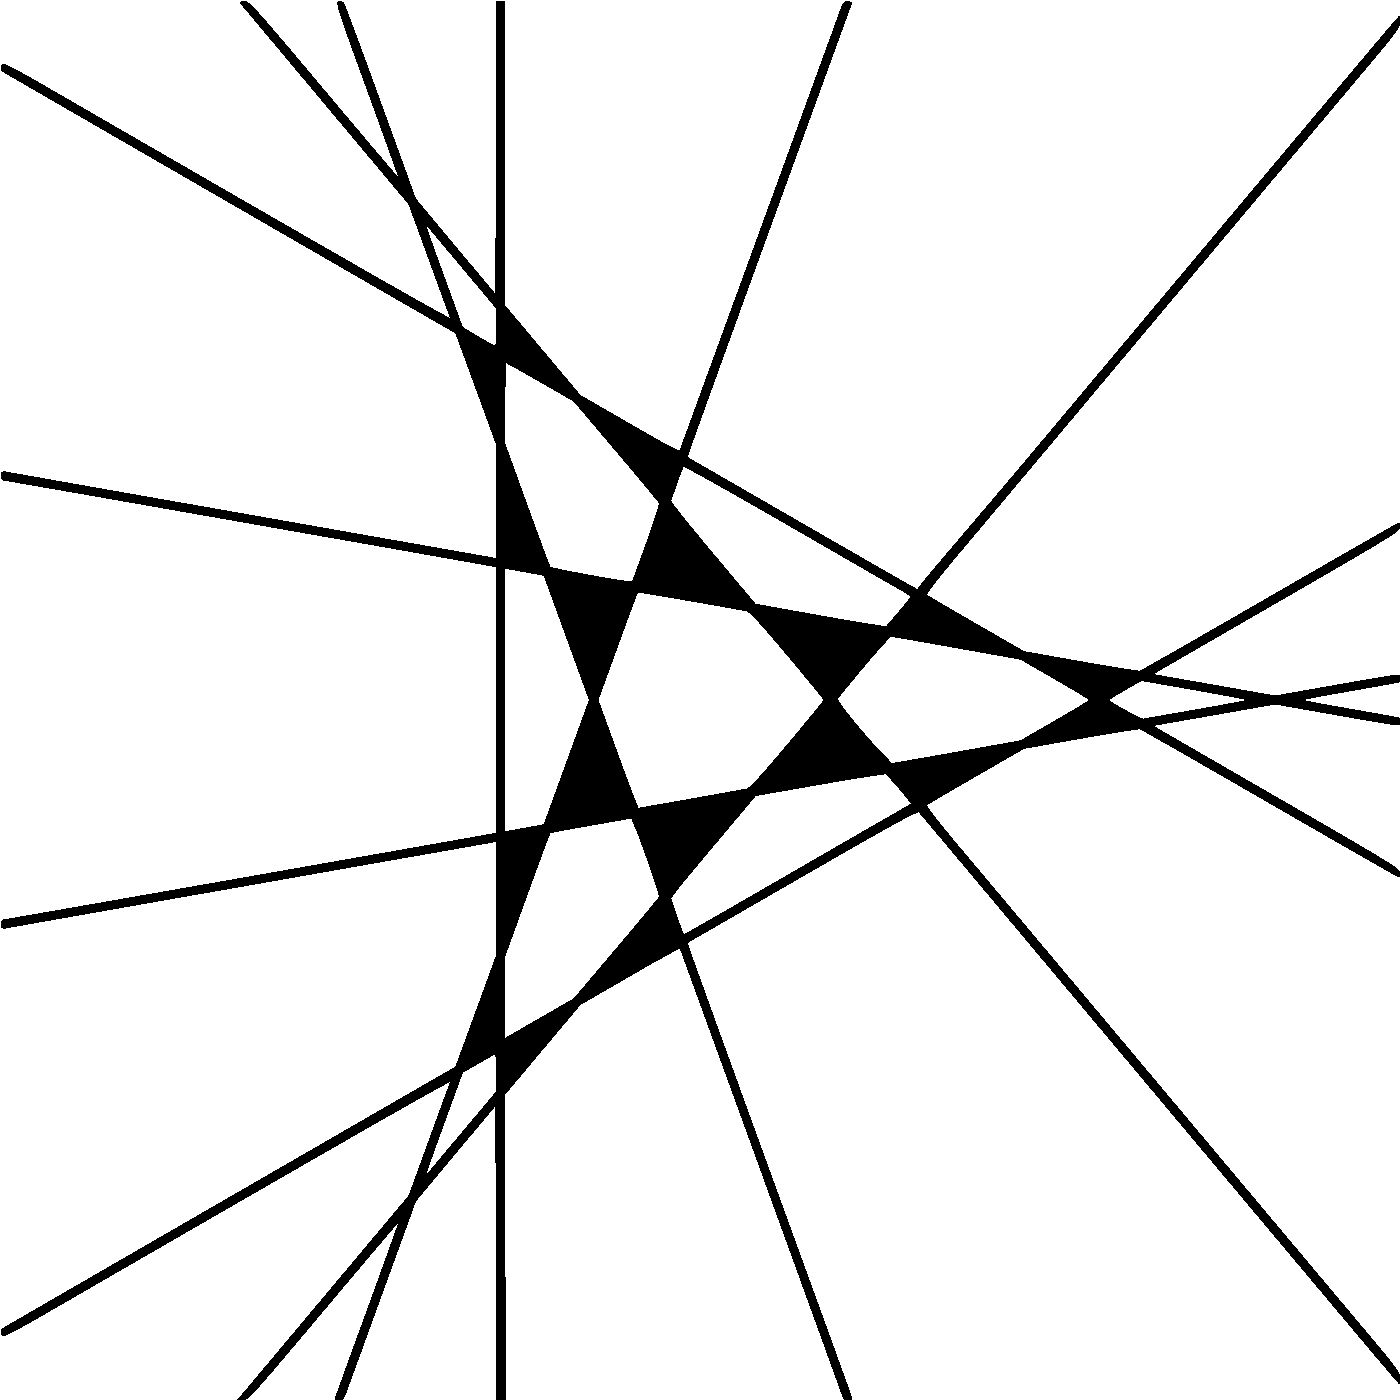
\includegraphics[height=1.5cm]{vielesing.pdf}
        &
        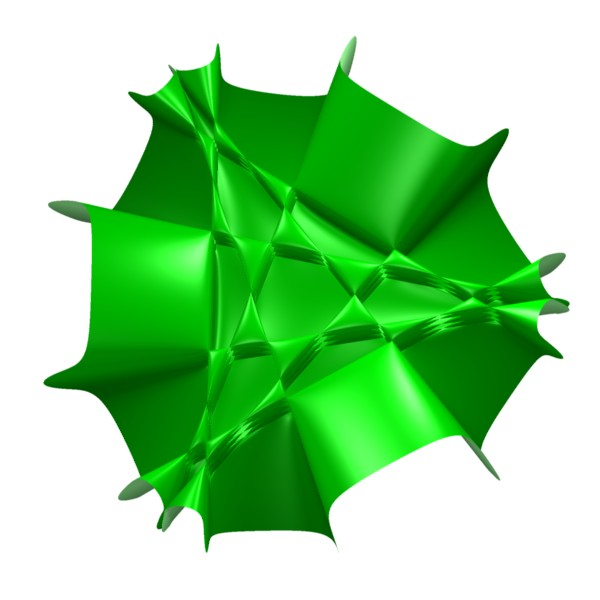
\includegraphics[height=1.5cm]{p9surface_von_oben}
      \end{tabular}
    \end{center}
\end{surferPage}
